\documentclass[9pt,a4paper]{article}
\usepackage[utf8]{inputenc}       
\usepackage[english,russian]{babel}
%\usepackage{PTSerif}                
\usepackage[pdftex]{graphicx}        
\usepackage{layout}                   
\usepackage{fancyhdr}                  
\usepackage{fullpage}                   
\usepackage{array}                       
\usepackage{longtable}                    
\usepackage{listings}
\usepackage{footnote}                       
                                             
\setlength\voffset{-1in}                      
\setlength\hoffset{-1in}                       
\setlength\topmargin{1cm}                       
\setlength\oddsidemargin{2cm}                    
\setlength\textheight{25.7cm}                     
\setlength\textwidth{17.001cm}                     
\setlength{\topskip}{1.3cm}                         
\setlength\headheight{0cm}                           
\setlength\headsep{0cm}                               
                                                       
\pagestyle{fancyplain}                                  
\fancyhf{}                                               
\cfoot{\small\em \textcopyright \hspace{0.1em} ARCСN 2013}
\rfoot{\small \thepage}

\renewcommand{\labelitemii}{$\circ$}
                                      
\title{Описание HCProbe}
\author{Александр Вершилов}

\begin{document}
\maketitle
\begin{figure}[!h]
   \centering 
   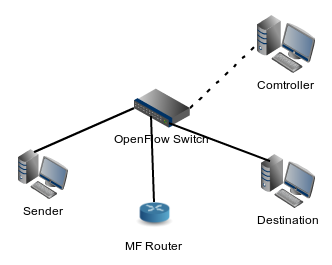
\includegraphics[width=0.3\columnwidth]{images/testcfg2.png}
\end{figure}                                                        

\tableofcontents

\pagebreak
\section{Общее описание}
HCProbe программа для реализиции софтового OpenFlow свича и простой
генерации разбору OpenFlow сообщений.

\section{EDSL}
\subsection{Структура программы}
\subsection{Создание свича}
Свич создается командами \lstinline!switch! или \lstinline!switchOn! в первом случае
в качестве образца будет использован свич с конфигурацией по умолчанию, во-втором 
переданный свич. Таким образом командой \lstinline!switchOn! можно скопировать свич.

\begin{lstlisting}
    switch <switchIP> $ do ..
\end{lstlisting}

\subsubsection{Настройка возможностей свича}

Настройки свича проводятся в окружении \lstinline!features!, в котором можно задать
возможности свича.

\begin{lstlisting}
    switch <switchIP> $ do
      features $ do
        ..
\end{lstlisting}

Внутри настроек возможностей свича можно добавить порты командой \lstinline!addPort!.

Команда \lstinline!addMACs! добавляет список маков к свичу, при этом маки разделяются
поровну между портами.

\lstinline!clearMACs! удаляет все маки добавленные к свичу.


\subsection{Запуск свича}
\subsection{Выполнение программы}
Полсле запуска  свича он начианет выполнять переданную ему программу, данный блок 
является обычным блоком haskell кода, который может взаимодействовать со свичем
используя дополнительные команды.

\lstinline!hangOn! ожидать вечно, может быть полезно в случае если нужно тестировать
свич.

\lstinline!waitForType! ожидание определенного типа сообщения: выполнение прогаммы
будет прервано то тех пор, пока не придет сообщение указанного типа, возвращает 
полученное сообщение.

\lstinline!waitForBID! ожидание сообщения с указанным значением \texttt{buffer id}.
Возвращшает полученное сообщение.

Для генерации сообщений желательно чтобы используемые номера транзакций и буфферов 
не пересекались, для этого служат команды \lstinline!nextBID! и \lstinline!nextTID!.

\subsubsection{Отправка сообщений}

\lstinline!send!

\lstinline!sendOFPacketIn!

\lstinline!sendARPGreeting!

\subsection{Изменение поведения по умолчанию}

\lstinline!setUserHandler!

\section{Приложения}
\subsection{Шаблоны программирования}
\subsubsection{Ожидание нескольких сообщений}

\begin{lstlisting}
import Control.Concurrent.Async

race_ action1 action2
\end{lstlisting}

\subsection{Примеры программ}

\end{document}
